\chapter{Conclusions}
\label{chap:Conclusions}
Defense against nuclear terrorism relies upon the ability to accurately detect and identify Special Nuclear Material (SNM).
The current standard for neutron detection in portal monitors is \iso[3]{He}, which is a diminishing resource. 
A significant amount of research is then focused on developing new (or optimizing an existing) neutron detection system to serve as a replacement RPMs.

Thin (less than approximately \SI{150}{\um}) polymeric films loaded with \iso[6]{Li} films or \iso[6]{Li} loaded ZnS:Ag scintillators show promise in meeting the criteria for replacement detectors; namely a 1) neutron interaction rate greater than 2.5 per nanogram \iso[252]{Cf} (in a specified test configuration) 2) an intrinsic gamma ray detection efficiency of less than one in a million in a 10 mR/hr field, and 3) the neutron and gamma efficiencies should not change by more than 10\% in a 10 mR/hr gamma field.
Design of a replacement detector technology capable of meeting these criteria needs to account for neutron interaction used for detection, the subsequent energy deposition  of the reaction products into the material, the scintillation that results from the energy deposition, and the transport of photons from the interaction site to the photomultiplier tube.
Understanding these complex reactions involve understanding the mechanisms of scintillation, light transport, and energy deposition while developing techniques to confirm simulations and confirm the light yield,intrinsic efficiency and count rate for the different detector materials.

\section{Neutron - Gamma Discrimination}
This work presented in this thesis outlines an approach in which a detector material is first characterized for it's ability to meet a gamma ray detection efficiency of less than one in a million. 
A pulse height discriminator is implemented as a mathematical lower level discriminator (MLLD) in which counts that are above a given channel number are counted as neutron counts, and counts below are discarded.
MCNPX simulations where used to establish the photon fluence over samples mounted on a PMT exposed to a 10 mR/hr field, allowing for the count rate per particle crossing to be established.
The MLLD is then determined as the discriminator setting in which for every million photons that cross the detector only one is counted.

The origination of the neutron - gamma discrimination in primary in film thickness as the scintillators tested for replacement detector criteria are low - z materials.
The thickness of the film impacts the discrimination firstly through the interaction rate (the interaction rate for photons in a given thickness of material can be expressed as $1-\exp\left(-(\mu/\rho)x \right )$), but for a \SI{1}{\MeV} photon in polystyrene to have an interaction rate of less than one in a million would require that the film be less than \SI{0.15}{\um}.
A far greater impact on the neutron - gamma discrimination comes from the range of the secondary electrons produced by Compton scattering in gamma-photon events and their energy deposition.
The electrons from the gamma interactions generally have energies on the order of 100 keV, while energies from the charged particle reactions of the neutrons have energies or the order to 10 keV.
Thus, the neutron reaction product energies tend to deposit more energy in the film than their gamma produced counterparts.
It is the the poor energy deposition by the electrons generated from photon events that allow for films to be much thicker than the thickness predicted based on the interaction rate.

Effective design must account for the energy deposition in the material, including the pulse height deficit of the impingement particle.
For example, the range of the alpha created in a \iso[6]{Li} neutron absorption is six times less than that of the triton, but the triton creates almost six times more photons than the alpha.
Simulations were completed using the GEANT4 toolkit to simulate the energy deposition of \iso[6]{LiF} loaded polystyrene
The average energy deposited was computed for each thickness and normalized by the incident energy for gammas by the Q-value of the reaction for neutrons, and is presented in Table ~\ref{tab:ConclusionFractionEDep}.
For thickness greater than \SI{150}{\um} there is little benefit in increasing the thickness of the film in terms of energy deposition by neutrons, since over 90\% of the energy is being deposited in the film, thus there is little reason to fabricate films thicker than \SI{150}{\um} because it allows for a greater percentage of energy to be deposited from gammas, resulting in a higher MLLD setting.
\begin{table}[ht]
    \caption{Fractional Energy Deposition for Various Thickness}
	\centering
	\begin{tabular}{c | c c}
	Thickness & Gamma Fraction & Neutron Fraction \\
	\hline
	\hline
	\SI{15}{\um} & 0.010 & 0.531 \\
	\SI{25}{\um} & 0.013 & 0.634 \\
	\SI{50}{\um} & 0.017 & 0.782 \\
	\SI{150}{\um} & 0.032 & 0.927 \\
	\SI{300}{\um} & 0.052 & 0.964 \\
	\SI{600}{\um} & 0.087 & 0.982 \\
	\SI{1}{\mm} & 0.130 & 0.989 \\
	\SI{1}{\cm} & 0.425 & 0.998 \\
	\end{tabular}
  \label{tab:ConclusionFractionEDep}
\end{table}

\section{Film Placement}
A single film does not have an adequate neutron count rate to satisfy the neutron detector requirements of 2.5 cps per nanogram \iso[252]{Cf} in a source that is \SI{2}{\m} from the detector midpoint, shielded by \SI{0.5}{\cm} of lead and moderated by \SI{2.5}{\cm} of high density polyethylene.
Layering the detectors, however, has been shown to improve the neutron count rate while maintaing the necessary gamma intrinsic detection efficiency.
A simple repeated layer design was first proposed as a solution to this problem, but due to the changing neutron flux through the detector is was quickly discarded as non-ideal.
The repeated layered detector design caused the neutron flux to never thermalize appreciably after being depleted by the first few detector slices; as neutrons became thermalized they would be captured by \iso[6]{Li}.
However, in the interior of the repeated layered detector design did not allow for any buildup, leading to waste of the absorber.
A more efficient use of the neutron detector material would be to space the material out in the detector, separating the layers with moderator, such that the neutron flux could be thermalized before the next detector layer.

Genetic algorithms were employed to optimize a binary model of the detector for the optimal geometry that had the highest count rate while using the least amount of absorber and still meeting the detection efficiency criteria.
This model consisted of using a binary representation of the layered detector geometry (where each layer is either a \verb+1+ (signifying a detector slice) or \verb+0+ (moderator slice).
The model was then evaluated using MCNPX and XSDRN to simulate the expected neutron interaction rate performance.

The position of the slices necessary for having the best usage of the absorber material while still maintaining the neutron count rate necessary for the criteria are then determined by the genetic algorithm.
\autoref{tab:GAOptRXNRate} shows the optimal geometry representation necessary to achieve a minimum of 2.5, 5.0 and 7.5 interactions per second per nanogram \iso[252]{Cf}.
These geometries are translated into positions of the right hand boundary of the material in \autoref{tab:OptGeoDetailed75},\autoref{tab:OptGeoDetailed5}, and \autoref{tab:OptGeoDetailed25}; annotated MCNPX renderings are shown in \autoref{fig:RPMLayeredRendering25} and \autoref{fig:RPMLayeredRendering5}, and \autoref{fig:RPMLayeredRendering75}.
\begin{table}
	\caption[Optimal geometry for various interaction rates]{Optimal genome geometries for various minimium interactions rates per nanogram \iso[252]{Cf}. The detector and simulation is configured per the PNNL criteria.}
	\label{tab:GAOptRXNRate}
	\begin{tabular}{m{7cm} m{5cm} m{2cm} }
	\toprule
	Genome & Interaction Rate & Mass \iso[6]{Li} \\
	\midrule
	01111101110100001000 & 7.56 & \SI{41.2}{\gram} \\
	011101001000000 & 5.31 & \SI{21.0}{\gram} \\
		0011010000 & 3.82 & \SI{12.6}{\gram} \\
	\bottomrule
	\end{tabular}
\end{table}
% Optimal geometry tables.  All are PS Films
begin{table}
	\caption[Optimal Layered Film Geometry for 7.5 interaction per second per nanogram Cf-252]{Optimal layered film geometry for an interaction rate of 7.5 interactions per second per nano-gram \iso[252]{Cf} in a 10\% \iso[6]{Li} loaded PS film. The positions shown in the table are the right boundary, where the detector starts at \SI{0.0}{\cm}. The genome representing this geoemtry is \protect\verb+01111101110100001000+}
	\label{tab:OptGeoDetailed75}
	\begin{tabular}{m{3cm} m{4cm}}
	\toprule
	Edge Position (\si{\cm}) & Material \\
	\midrule
0.635&Moderator\\
0.645&Detector\\
1.270&LightGuide\\
1.280&Detector\\
1.905&LightGuide\\
1.915&Detector\\
2.540&LightGuide\\
2.550&Detector\\
3.175&LightGuide\\
3.185&Detector\\
3.810&LightGuide\\
4.445&Moderator\\
4.455&Detector\\
5.080&LightGuide\\
5.090&Detector\\
5.715&LightGuide\\
5.725&Detector\\
6.350&LightGuide\\
6.985&Moderator\\
6.995&Detector\\
7.620&LightGuide\\
8.255&Moderator\\
8.890&Moderator\\
9.525&Moderator\\
10.160&Moderator\\
10.170&Detector\\
10.795&LightGuide\\
11.430&Moderator\\
12.065&Moderator\\
12.700&Moderator\\
	\bottomrule
	\end{tabular}
\end{table
\begin{table}
	\caption[Optimal Layered Film Geometry for 5.0 interaction per second per nanogram Cf-252]{Optimal layered film geometry for an interaction rate of 5.0 interactions per second per nano-gram \iso[252]{Cf}  in a 10\% \iso[6]{Li} loaded PS film. The positions shown in the table are the right boundary, where the detector starts at \SI{0.0}{\cm}. The genome representing this geoemtry is \protect\verb+011101001000000+}
	\label{tab:OptGeoDetailed5}
	\begin{tabular}{m{3cm} m{4cm}}
	\toprule
	Edge Position (\si{\cm}) & Material \\
	\midrule
0.847&Moderator\\
0.857&Detector\\
1.693&LightGuide\\
1.703&Detector\\
2.540&LightGuide\\
2.550&Detector\\
3.387&LightGuide\\
4.233&Moderator\\
4.243&Detector\\
5.080&LightGuide\\
5.927&Moderator\\
6.773&Moderator\\
6.783&Detector\\
7.620&LightGuide\\
8.467&Moderator\\
9.313&Moderator\\
10.160&Moderator\\
11.007&Moderator\\
11.853&Moderator\\
12.700&Moderator\\
	\bottomrule
	\end{tabular}
\end{table}
\begin{table}
	\caption[Optimal Layered Film Geometry for 2.5 interaction per second per nanogram Cf-252]{Optimal layered film geometry for an interaction rate of 2.5 interactions per second per nano-gram \iso[252]{Cf} in a 10\% \iso[6]{Li} loaded PS film. The positions shown in the table are the right boundary, where the detector starts at \SI{0.0}{\cm}. The genome representing this geoemtry is \protect\verb+0011010000+}
	\label{tab:OptGeoDetailed25}
	\begin{tabular}{m{3cm} m{4cm}}
	\toprule
	Edge Position (\si{\cm}) & Material \\
	\midrule
1.270&Moderator\\
2.540&Moderator\\
2.550&Detector\\
3.810&LightGuide\\
3.820&Detector\\
5.080&LightGuide\\
6.350&Moderator\\
6.360&Detector\\
7.620&LightGuide\\
8.890&Moderator\\
10.160&Moderator\\
11.430&Moderator\\
12.700&Moderator\\
	\bottomrule
	\end{tabular}
\end{table

\begin{figure}
  \centering
  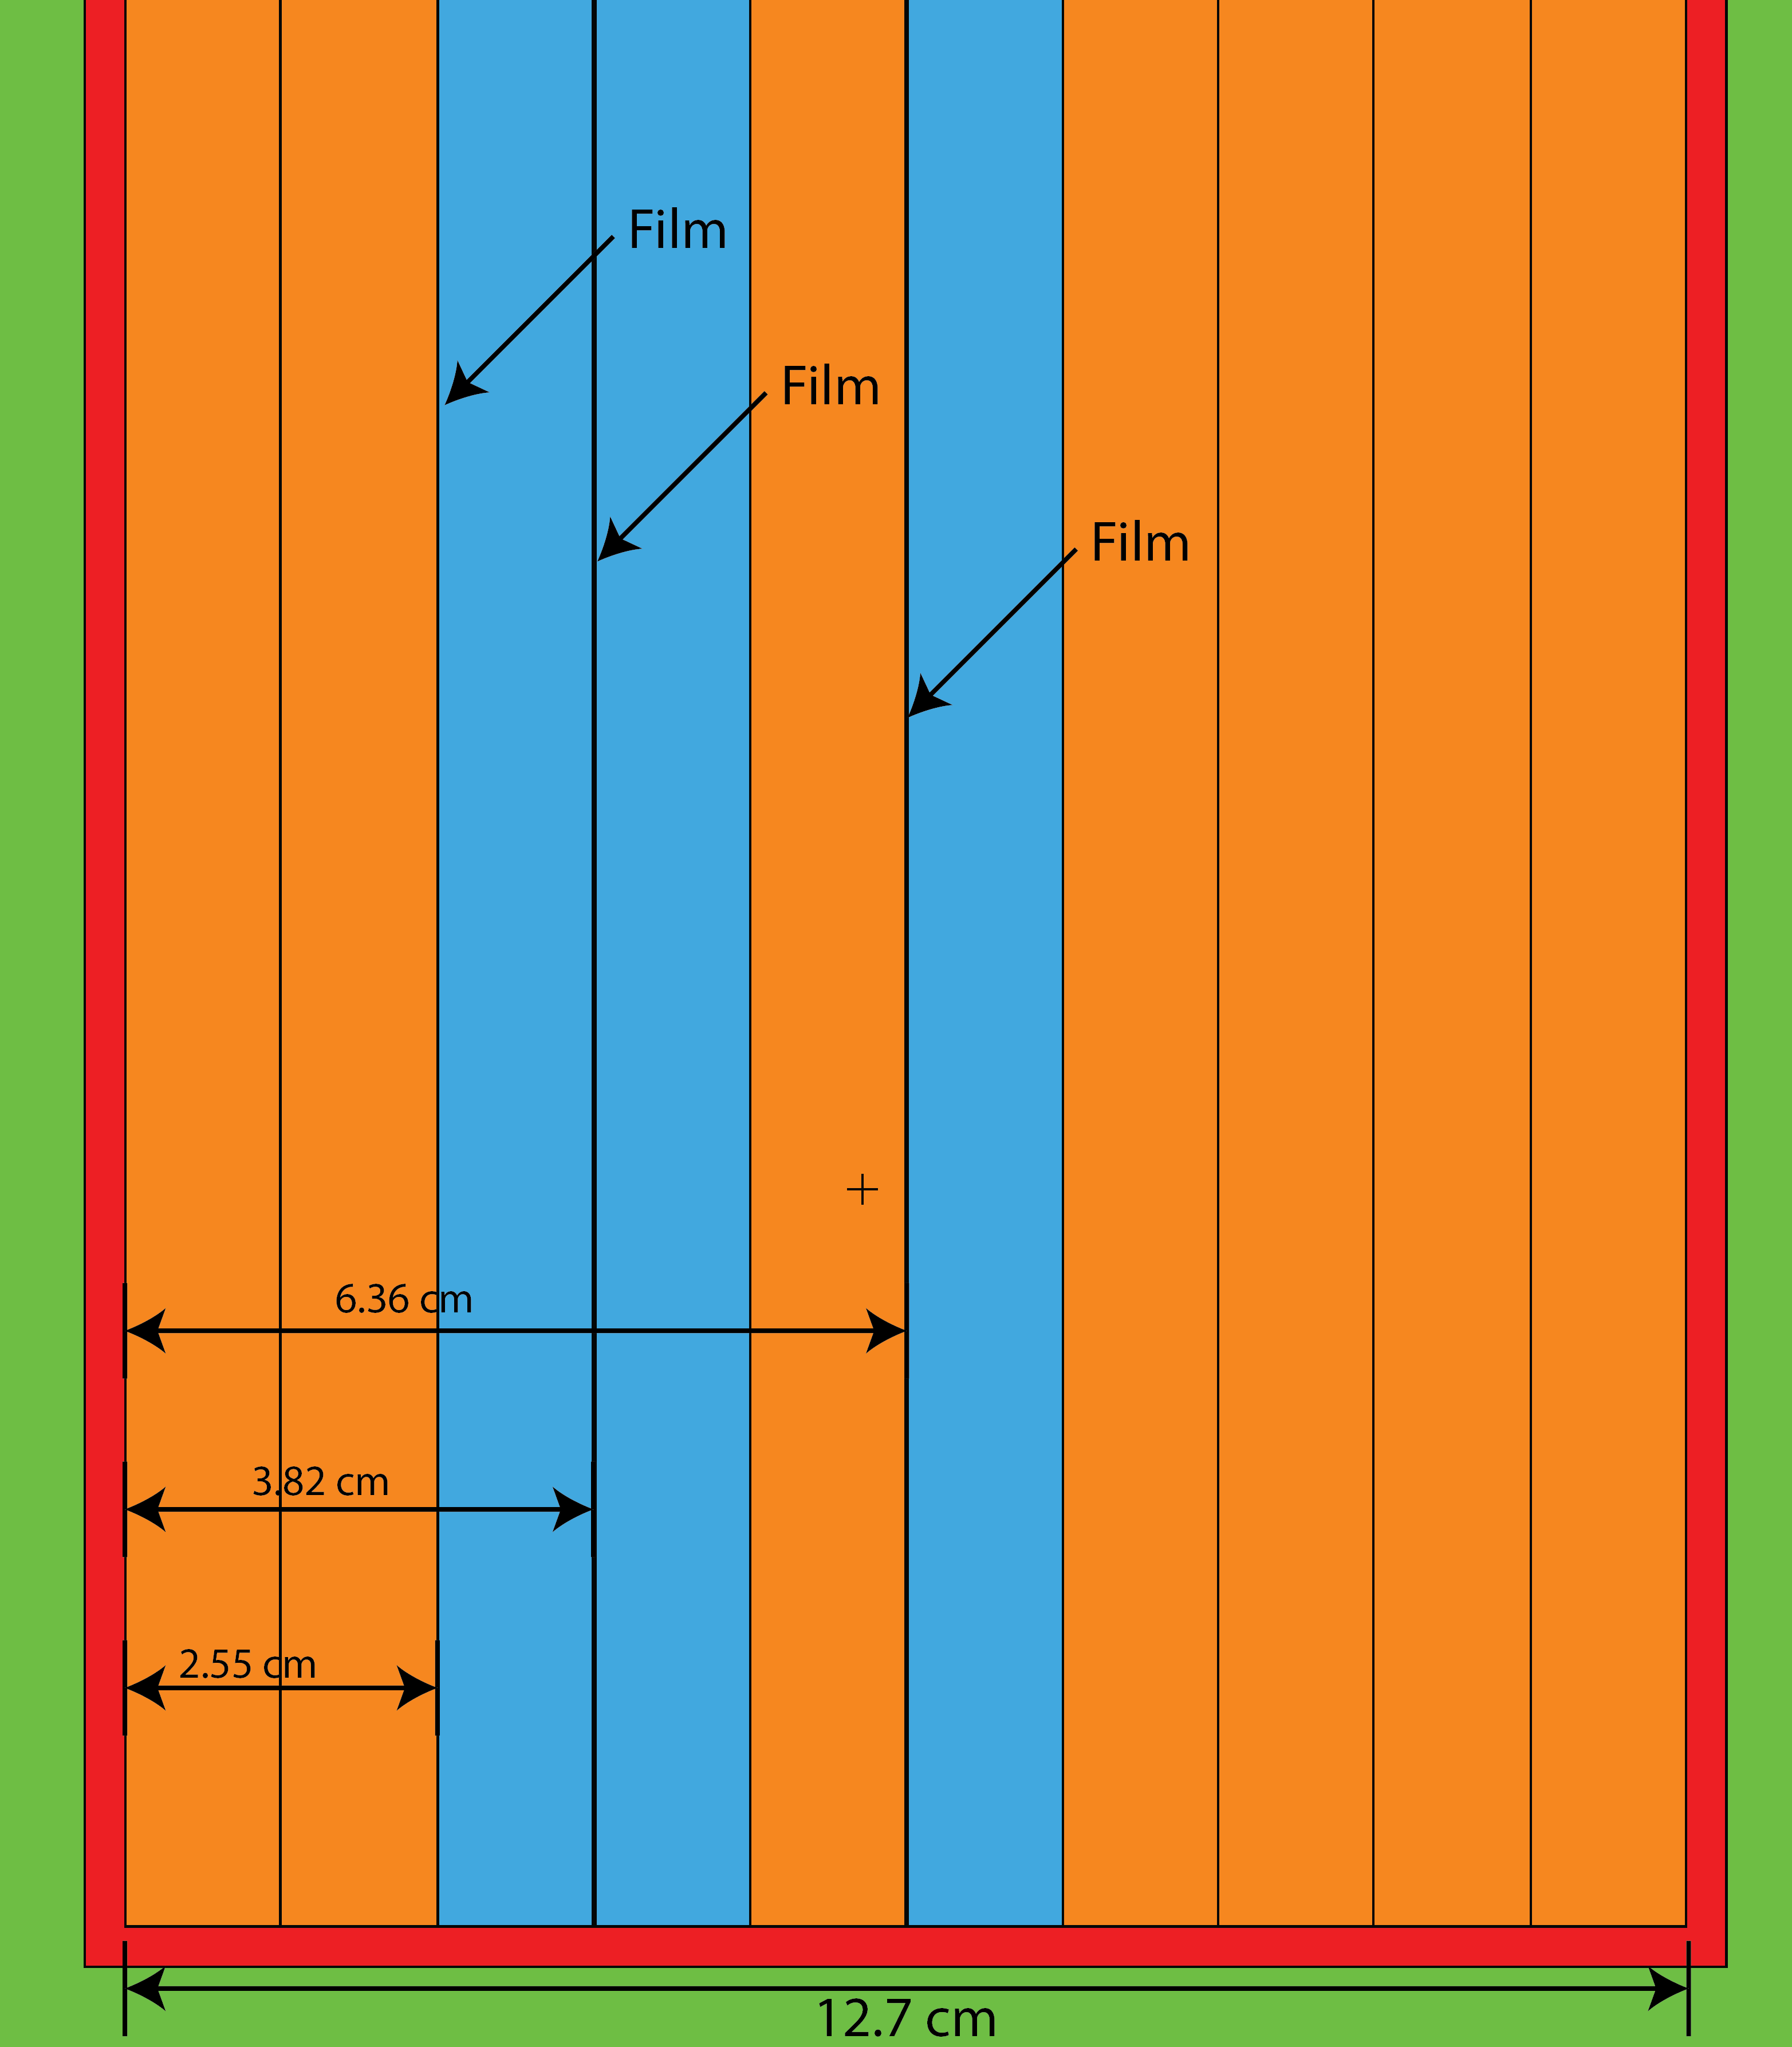
\includegraphics[width=\textwidth]{RPM8OptLayered_25cps}
  \caption[Position of Films in Optimized Layered RPM8 (2.5 intearctions per nanogram Cf-252)]{Position of 10\% \iso[6]{Li} loaded polystyrene films in  an RPM8. The minimum count rate achieved in this configuration is 2.5 interactions per second per nanogram \iso[252]{Cf}.}
  \label{fig:RPMLayeredRendering25}
\end{figure}
\begin{figure}
  \centering
  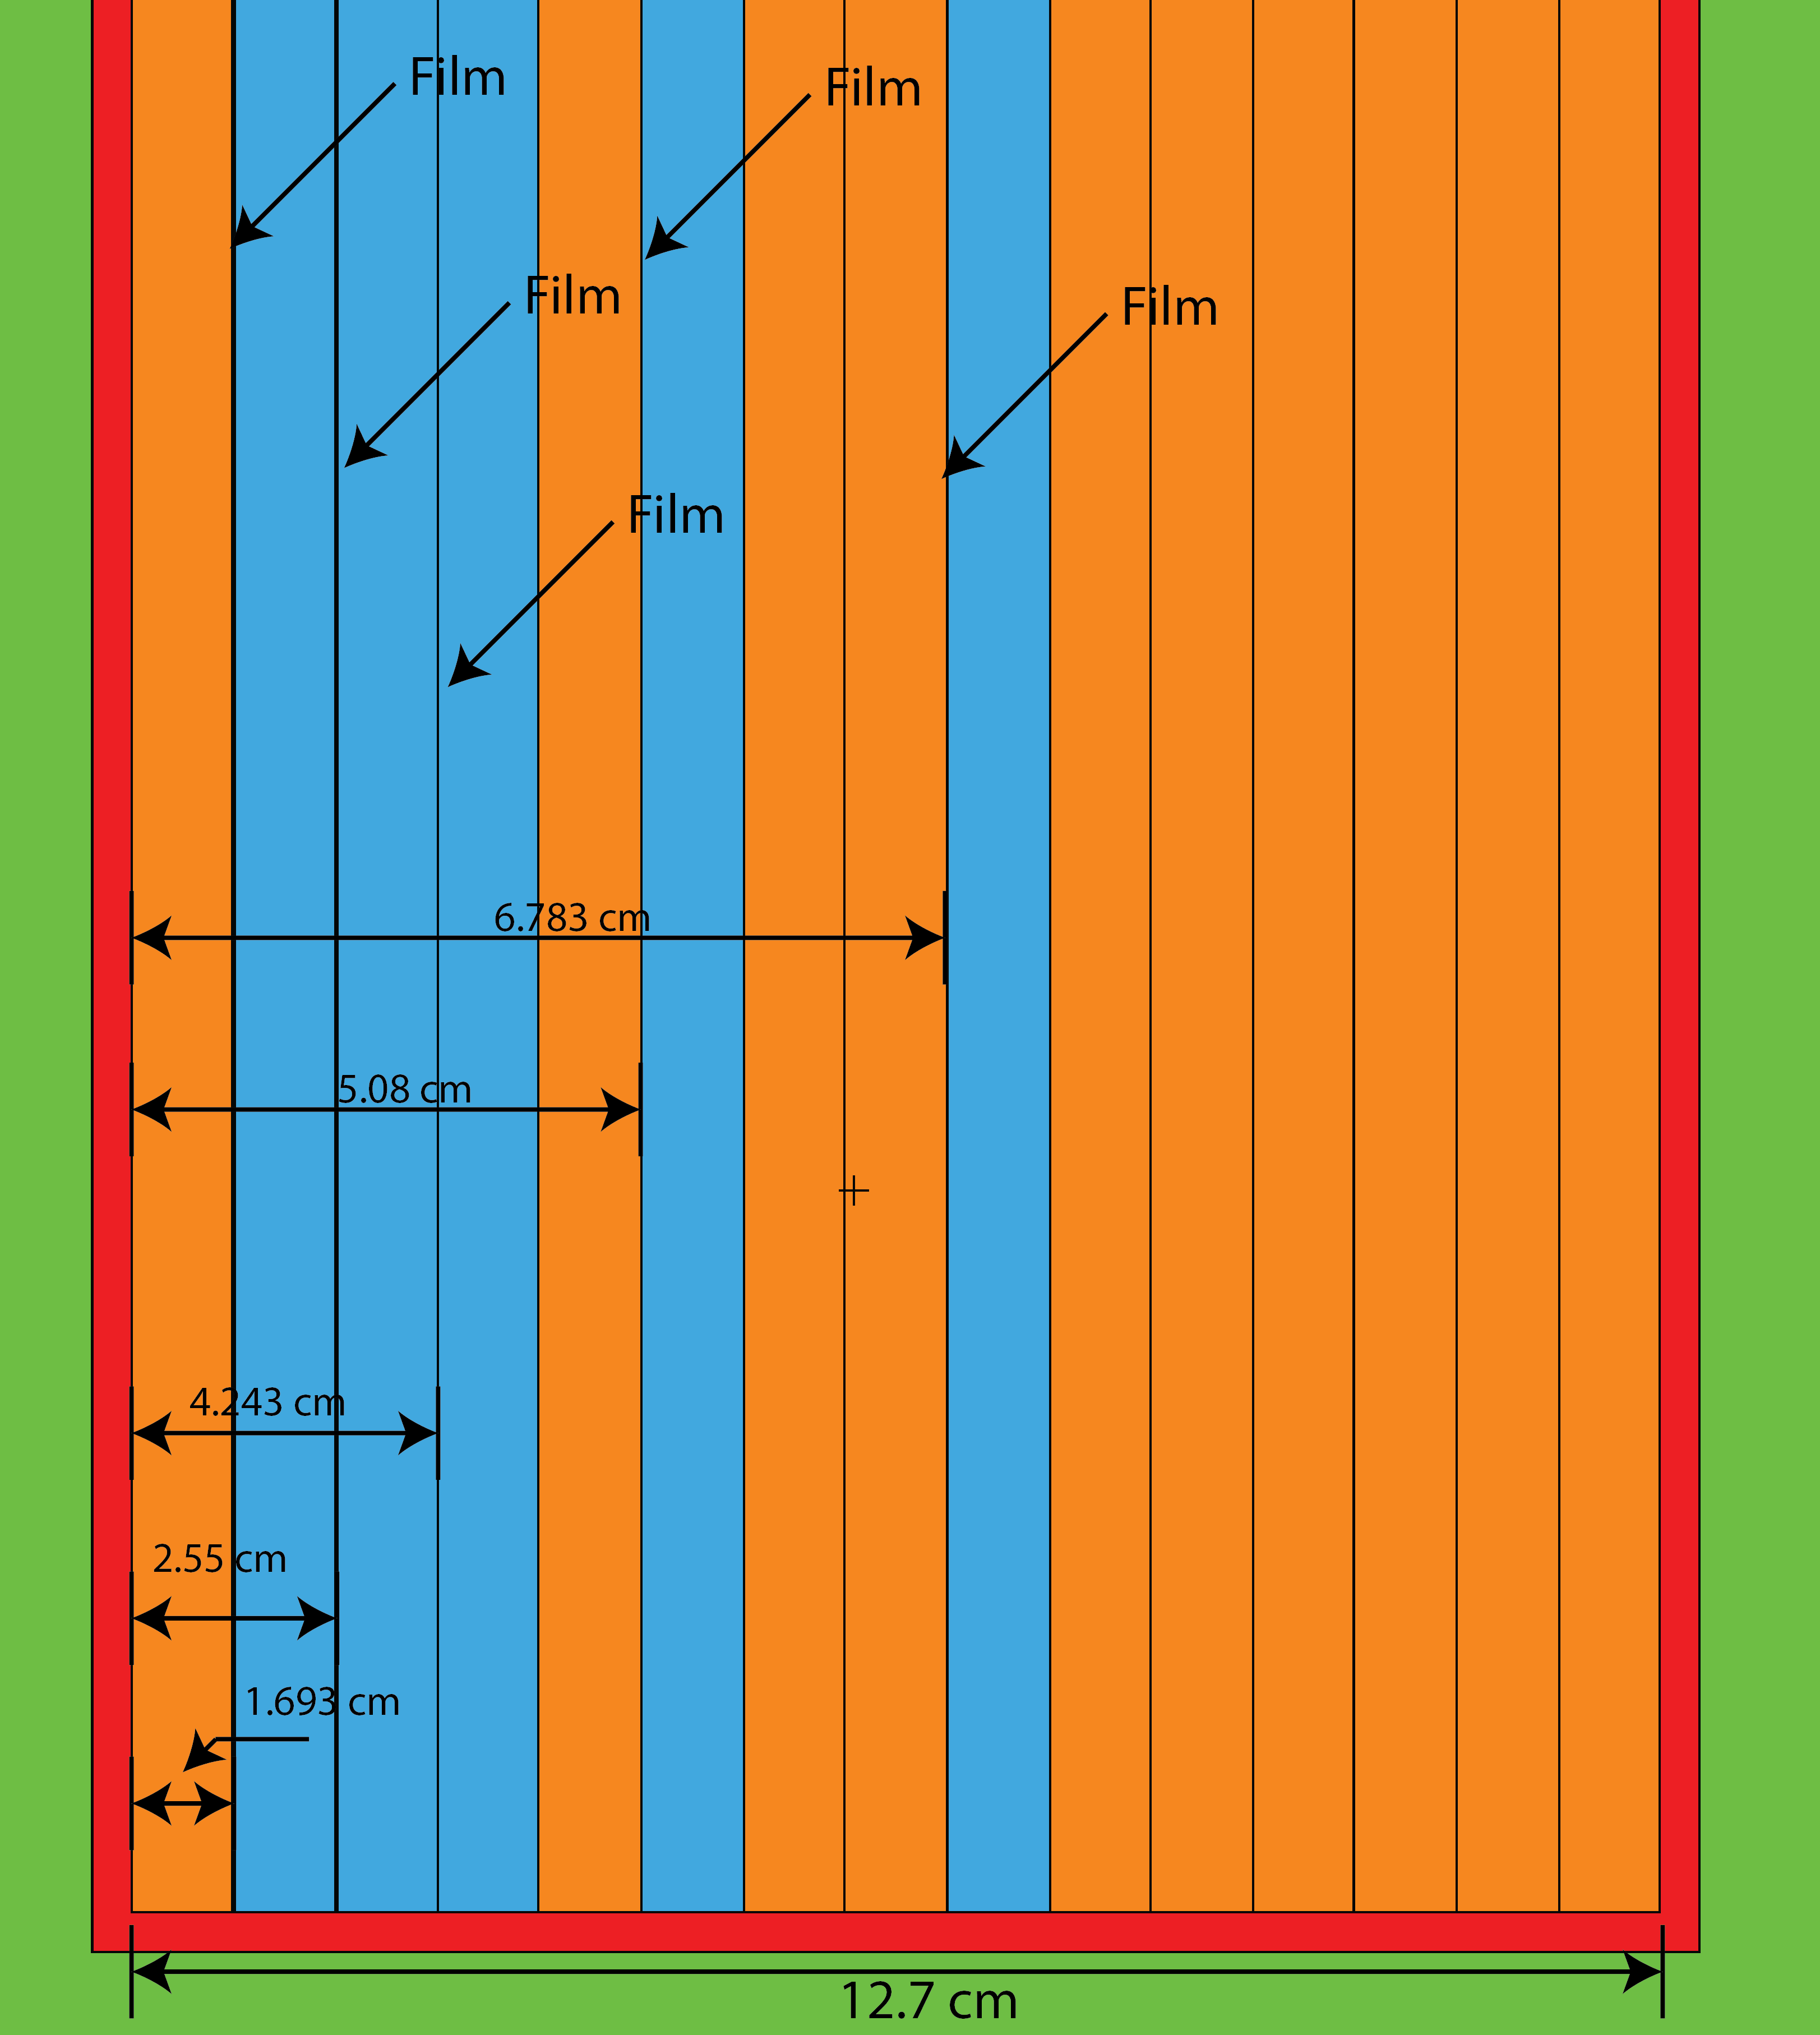
\includegraphics[width=\textwidth]{RPM8OptLayered_5cps}
  \caption[Position of Films in Optimized Layered RPM8 (5.0 intearctions per nanogram Cf-252)]{Position of 10\% \iso[6]{Li} loaded polystyrene films in  an RPM8. The minimum count rate achieved in this configuration is 5.0 interactions per second per nanogram \iso[252]{Cf}.}
  \label{fig:RPMLayeredRendering5}
\end{figure}
\begin{figure}
  \centering
  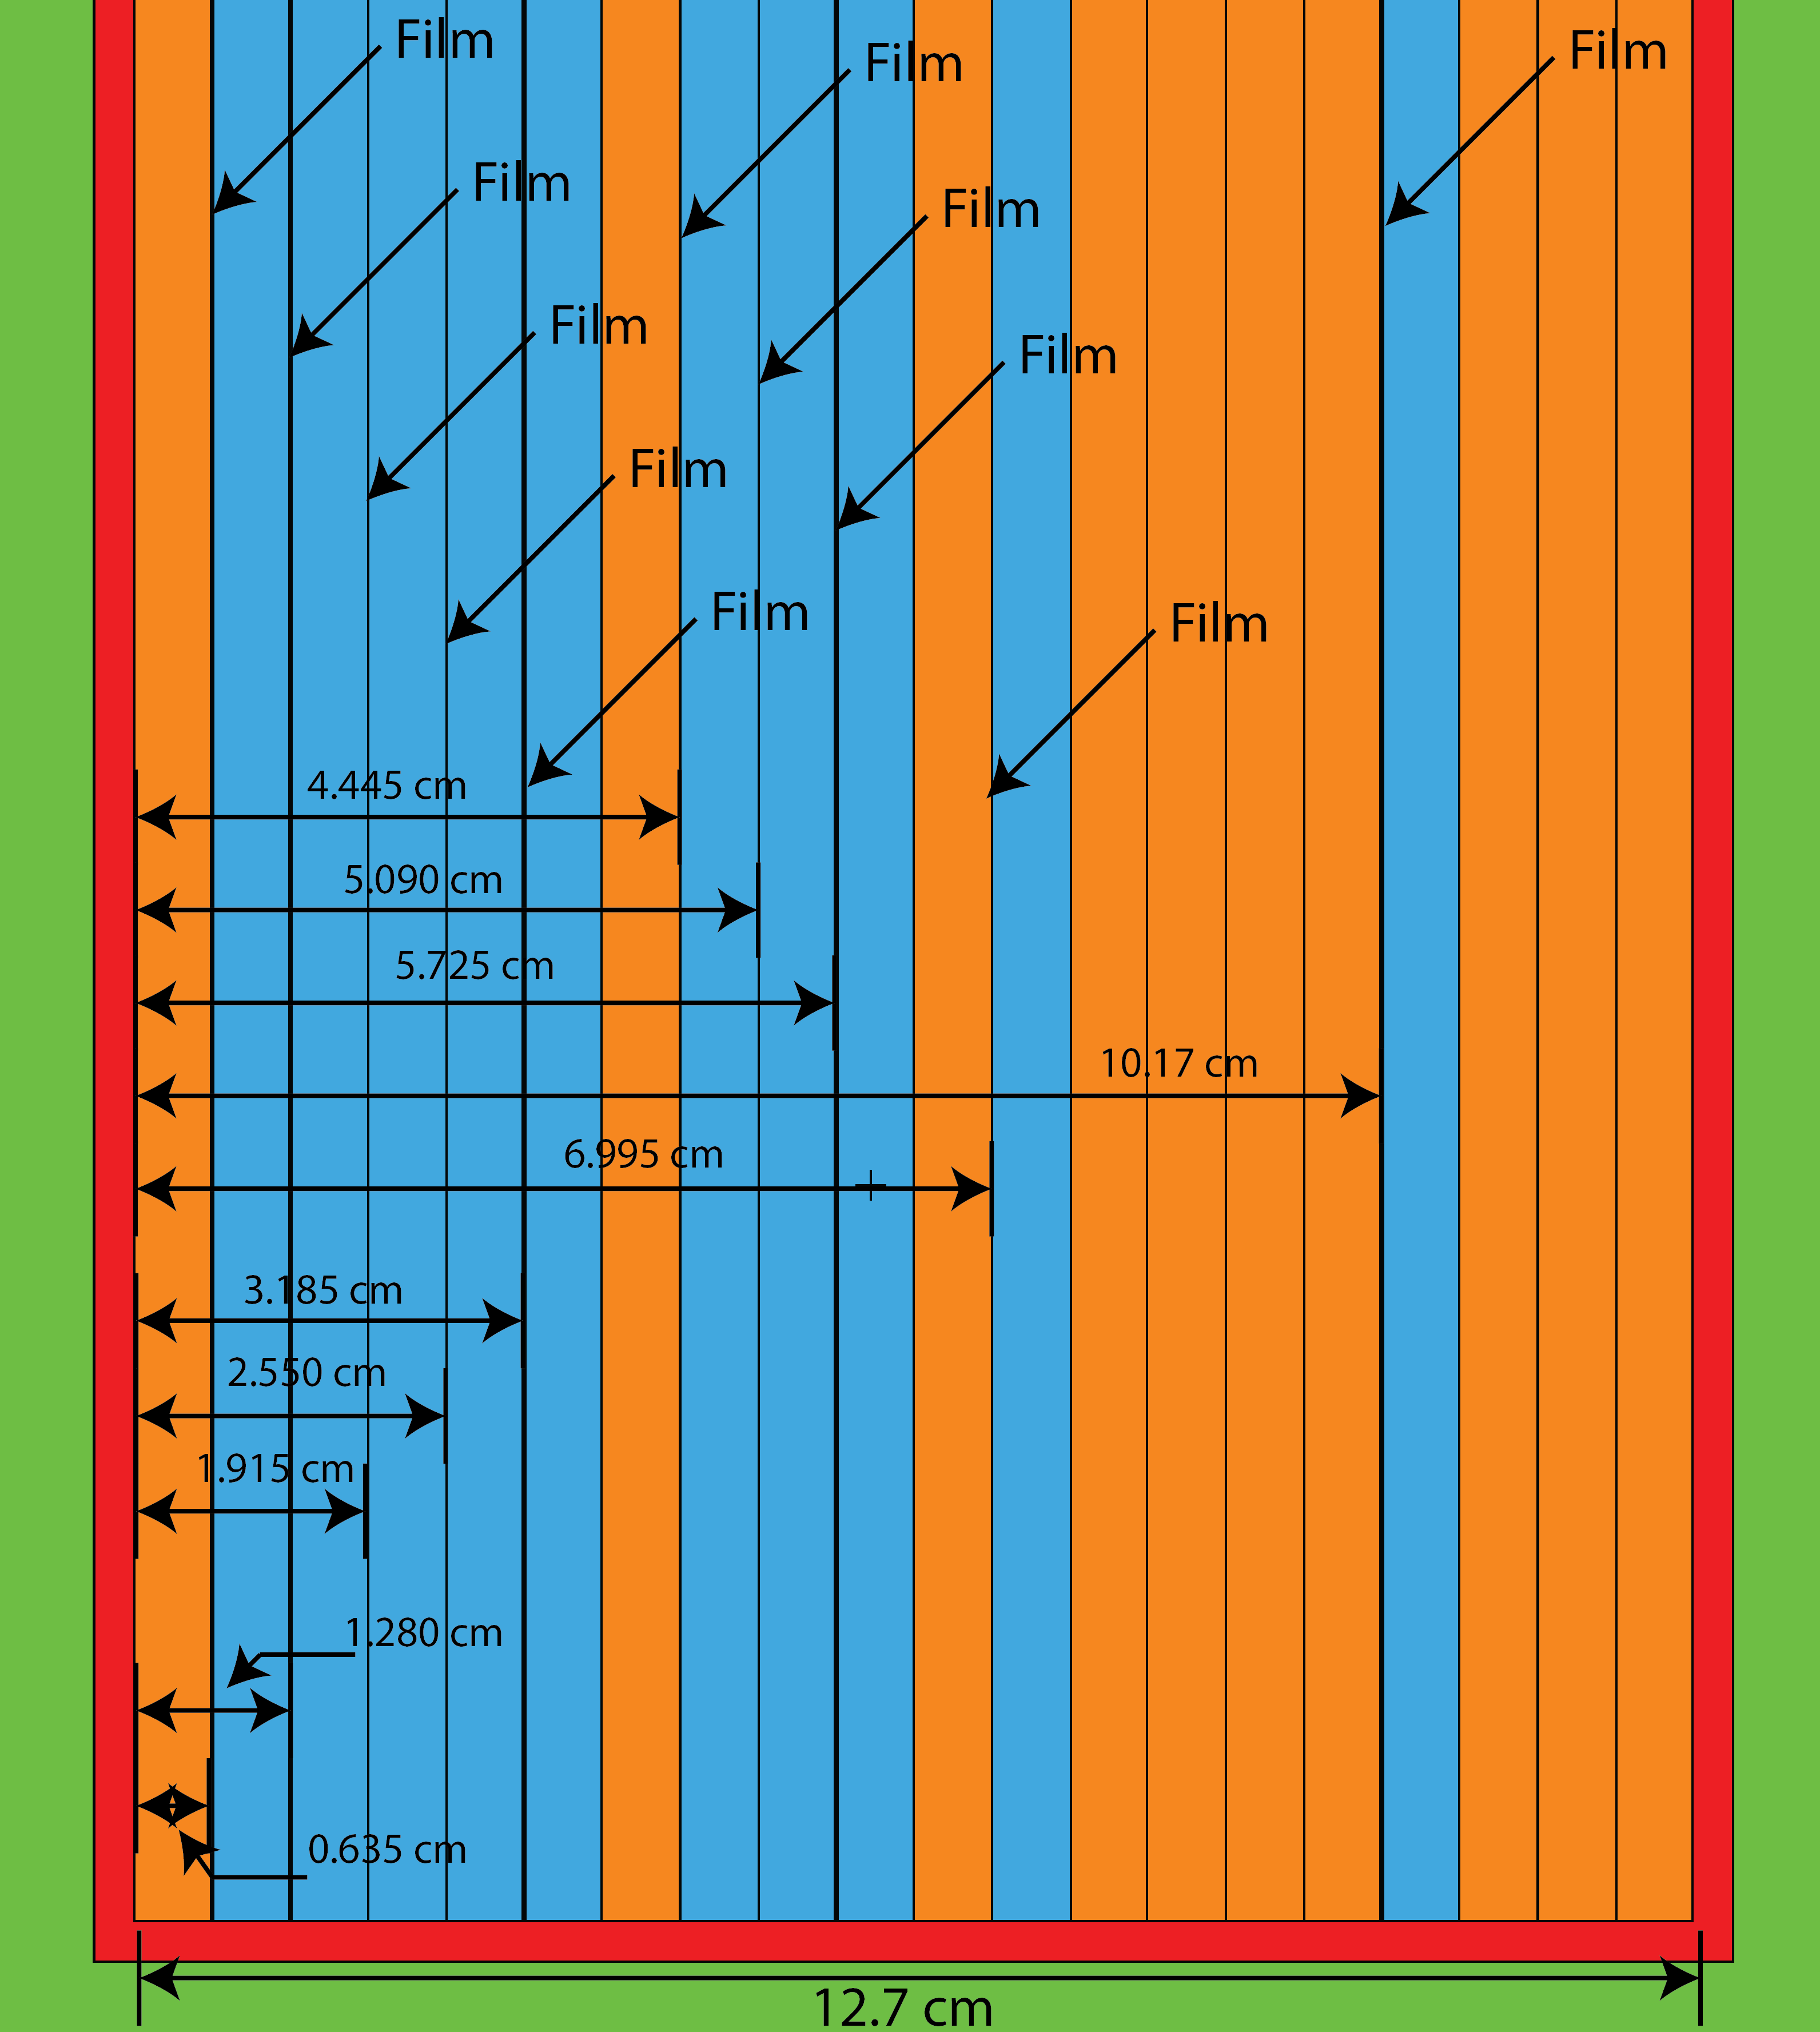
\includegraphics[width=\textwidth]{RPM8OptLayered_75cps}
  \caption[Position of Films in Optimized Layered RPM8 (7.5 intearctions per nanogram Cf-252)]{Position of 10\% \iso[6]{Li} loaded polystyrene films in  an RPM8. The minimum count rate achieved in this configuration is 7.5 interactions per second per nanogram \iso[252]{Cf}.}
  \label{fig:RPMLayeredRendering75}
\end{figure}

A physical basis of the optimal solution found by the genetic algorithm can be found by observing the form of the optimal solutions.
These solutions involve an initial moderator layer in order to ensure that all of the neutrons are thermalized.
After this moderator layer a film layer is placed to utilize this neutron spectra; however not all of the thermal neutrons are captured (as the mean free path of a neutron in polyethylene is about \SI{0.37}{\cm} and thus some pass through the material) and another absorber layer is needed to capture those neutrons.  
The neutron flux is then moderated again, and additional layers of detectors are needed to capture this neutron cross section.
However, it is desirably to have a large neutron reflector in the portal monitor to reflect neutrons back into the detector slices. 
Theoretically this reflector should be as large as possible, but the limited space of the RPM provides a constraint.

mathematical lower level discriminator 
This work will be novel in its utilization of high fidelity energy deposition to explain the origins of neutron-gamma discrimination through the range of secondary electrons from the neutron and photons reactions in their subsequent energy deposition.
The neutronic performance of a film will then be assessed by calculating the performance of a full scale replacement RPM in the test environment with MCNPX.
Non-linear search techniques will then be used to find the optimal geometry of the MCNPX model of the detector that best utilizes the neutron absorber.
Finally, the scintillation light from the detectors will be simulated with the GEANT4 toolkit, and the performance of the detector based upon the collected light signal reported.
Different light collection strategies will be employed to maximize the light collection efficiency and minimize the cost of electronics necessary for the detector.


A toolkit for the optimization of a radiation portal monitor has been presented in which simulations and measurements are combined to form a design suite.

\section{Neturon - Photon Discrimination}
Attention needs to be paid to the thickness of a film in order to maximize the neutron / photon discrimination that goes simply beyond the probability of interaction.

The choice of detector thickness must take this into account, and a balance struck.

